\chapter{Einrichten des SatNOGS Client}
\label{chap:gs-setup}
Der SatNOGS Client bildet das Herzstück der gesamten Empfangsstation. Er ist für die Ausführung und Koordinierung der mit der Empfangstation geplanten Observationen zuständig und bildet die Schnittstelle zur SatNOGS Datenbank. Das SatNOGS Client Script kann auf einer beliebigen Linux Distribution installiert und ausgeführt werden. In diesem Fall empfiehlt es sich für die Anwendung eines Rasperry Pi 4 Einplatinencomputers zur Ausführung des Client Scripts, das speziell für den SatNOGS Client entwickelte Raspbian SatNOGS Image zu verwenden. Dieses angepasste Image für das Raspbian Betriebssystem sorgt dafür, dass alle benötigten Softwarepakete und das SatNOGS Setup Script vorinstalliert sind und der SSH-Server auf dem Raspberry Pi 4 aktiviert wird. Auf die Installation wird nicht näher eingegangen, sondern auf die Anleitung im SatNOGS Wiki \cite{noauthor_raspberry_nodate} verwiesen. 

\section{Grundlegende Konfiguration}
\subsection{Verbinden zum Raspberry PI 4}
Um Einstellungen am Raspberry Pi 4 vornehmen zu können wird auf diesen über SSH zugegriffen. Dazu muss das Gerät, welches auf den Raspberry Pi 4 zugreift, am besten mit dem selben Netzwerk verbunden sein wie der Raspberry. Die einfachste Vorgehensweise, um sich mit dieser Voraussetzung mit einem Windows System zum Raspberry Pi 4 über SSH zu verbinden, besteht darin, in der Eingabeaufforderung den Befehl \glqq ssh *hostname*\grqq{} auszuführen. Der Hostname wird im Zuge der Installation des Raspbian SatNOGS Image vergeben und lautet in diesem Fall \glqq qfh\grqq{}. Wurde bei der Installation ein Passwort festgelegt, so erscheint anschließend eine Aufforderung dieses einzugeben. Nach der Eingabe wird bei erfolgreicher Verbindung folgende Information zurückgegeben:

\begin{figure} [H]
	\centering
	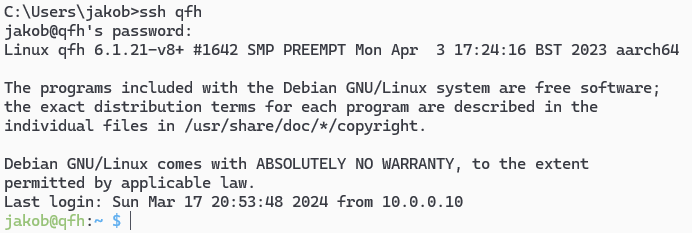
\includegraphics[width=\linewidth]{../ref/successfull_login.png}
	\caption{Erfolgreiche Verbindung über SSH}
	\label{fig:htrl-uhf(test)successfulllogin}
\end{figure}

\subsection{Hauptmenü}
Mithilfe des Befehls \glqq sudo satnogs-setup\grqq{} öffnet sich das Hauptmenü des SatNOGS Client, über welches alle Einstellungen vorgenommen werden können.

\begin{figure} [H]
	\centering
	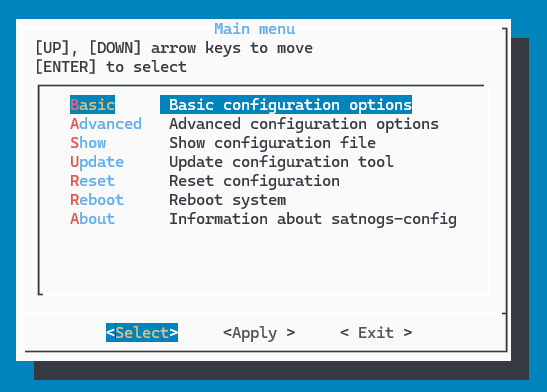
\includegraphics[width=.5\linewidth]{../ref/mainmenu.png}
	\caption{SatNOGS Client: Hauptmenü}
	\label{fig:mainmenu}
\end{figure}

Wurden alle Einstellungen vorgenommen, so können diese mit \glqq Apply\grqq{} angewendet und gespeichert werden.

\subsection{Einstellungen}
Wird im Hauptmenü der Reiter \glqq Basic\grqq{} mit \glqq Enter\grqq{} ausgewählt, erscheint folgendes Fenster über welches alle grundlegenden Einstellungen zum Betrieb einer Empfangsstation vorgenommen werden können.

\begin{figure} [H]
	\centering
	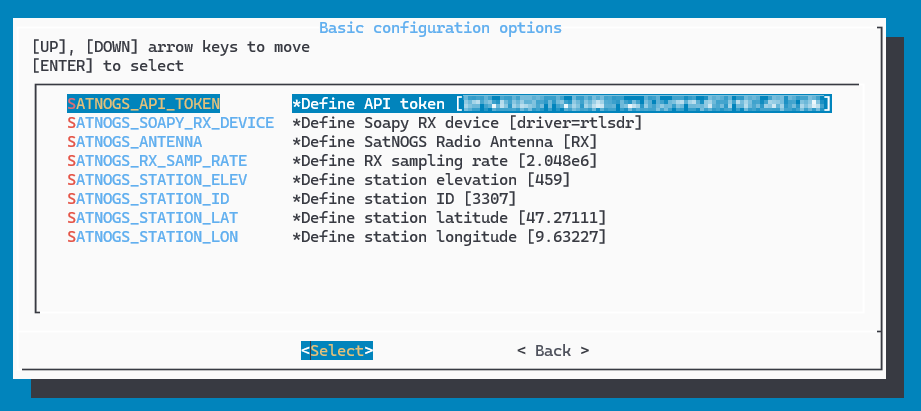
\includegraphics[width=.75\linewidth]{../ref/basic_configurations.png}
	\caption{SatNOGS Client: grundlegende Einstellungen}
	\label{fig:basic_configurations}
\end{figure}

\subsubsection{SATNOGS\textunderscore API\textunderscore TOKEN}
Der API-Schlüssel, welcher mit dem SatNOGS-Benutzerkonto verknüpft ist, wird zur Identifizierung sowie Authentifizierung gegenüber der SatNOGS-Datenbank benötigt. Er kann auf dem Benutzerprofil der SatNOGS-Netzwerk Webseite durch das Klicken auf den in der folgenden Grafik mit 1 markierten Button an der mit 2 markierten Stelle abgelesen werden.

\begin{figure} [H]
	\centering
	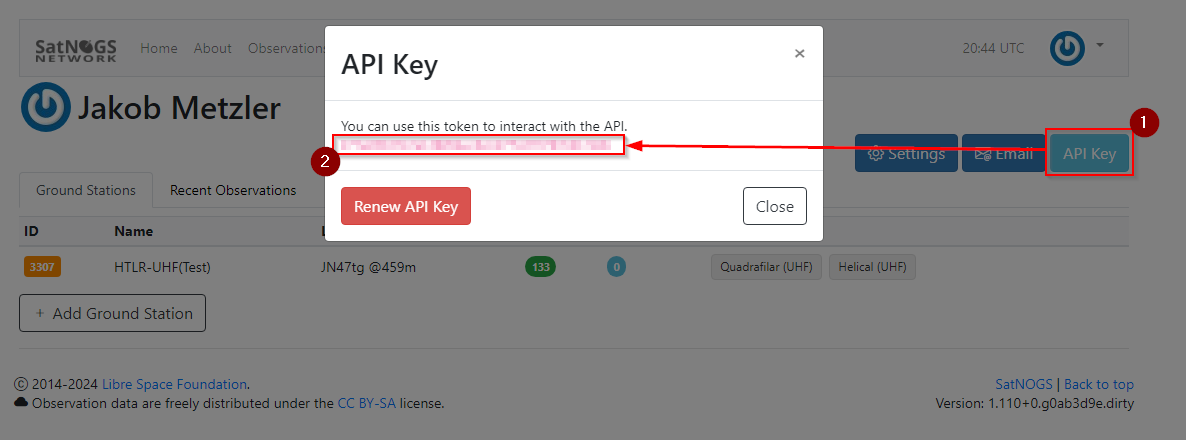
\includegraphics[width=.75\linewidth]{../ref/apitoken.png}
	\caption{SatNOGS-Netwerk Homepage: API-Schüssel ermitteln \cite{noauthor_satnogsdashboard_nodate}}
	\label{fig:apikey}
\end{figure}

\subsubsection{SATNOGS\textunderscore SOAPY\textunderscore RX\textunderscore DEVICE}
Mithilfe dieses Einstellungsparameters wird dem SatNOGS Client das verwendete SDR mitgeteilt. In diesem Fall entspricht das SDR dem, im Kapitel \ref{sec:sdr} genauer erläuterten, RTL-SDR Blog v3. Die dementsprechend einzugebende Treiber-Kennzeichnung lautet \glqq driver=rtlsdr\grqq{} \cite{noauthor_satnogsclient_nodate}. Weitere Treiber-Kennzeichnungen können auf der Software Defined Radio Seite des SatNOGS Wiki nachgeschlagen werden \cite{noauthor_software_nodate}.

\subsubsection{SATNOGS\textunderscore ANTENNA}
Über diesen Einstellungsparameter wird entsprechend dem verwendeten SDR und dem passenden Parameter der Modus des SDRs konfiguriert. Für das RTL-SDR Blog v3 entspricht das dem Parameter \textbf{RX} \cite{noauthor_satnogsclient_nodate}. Entsprechende Parameter für weitere SDR Typen können auf der Software Defined Radio Seite des SatNOGS Wiki nachgeschlagen werden \cite{noauthor_software_nodate}. 

\subsubsection{SATNOGS\textunderscore RX\textunderscore SAMP\textunderscore RATE}
Dieser Parameter legt die Abtastrate des SDRs fest. Für das RTL-SDR Blog v3 wird eine Abtastrate von 2.048 Megasamples pro Sekunde empfohlen \cite{noauthor_satnogsclient_nodate}, was über den Parameter 2.048e6 eingestellt werden kann. Auch hier finden sich für weitere SDRs Informationen auf der Software Defined Radio Seite des SatNOGS Wiki \cite{noauthor_software_nodate}. 

\subsubsection{SATNOGS\textunderscore STATION\textunderscore ELEV}
Für diesen Parameter ist es notwendig, die Höhenlage der Empfangsstation zu ermitteln. Dazu empfiehlt sich die Verwendung einer interaktiven topografischen Karte wie \url{http://www.de-at.topographic-map.com}. Der für den Standort der HTL Rankweil ermittelte Wert, welcher auch dem Parameter entspricht, beträgt 459 Meter. Dieser Wert wird für die Berechnungen der passierenden Satelliten und den dazugehörigen Elevation- und Azimutalwinkel verwendet.

\subsubsection{SATNOGS\textunderscore STATION\textunderscore ID}
Die Station-ID wird zur eindeutigen Identifikation der Empfangsstation im SatNOGS-Netzwerk verwendet. Sie kann auf der Seite des Benutzerprofils auf der Homepage des SatNOGS-Netzwerks abgelesen werden. 

\begin{figure} [H]
	\centering
	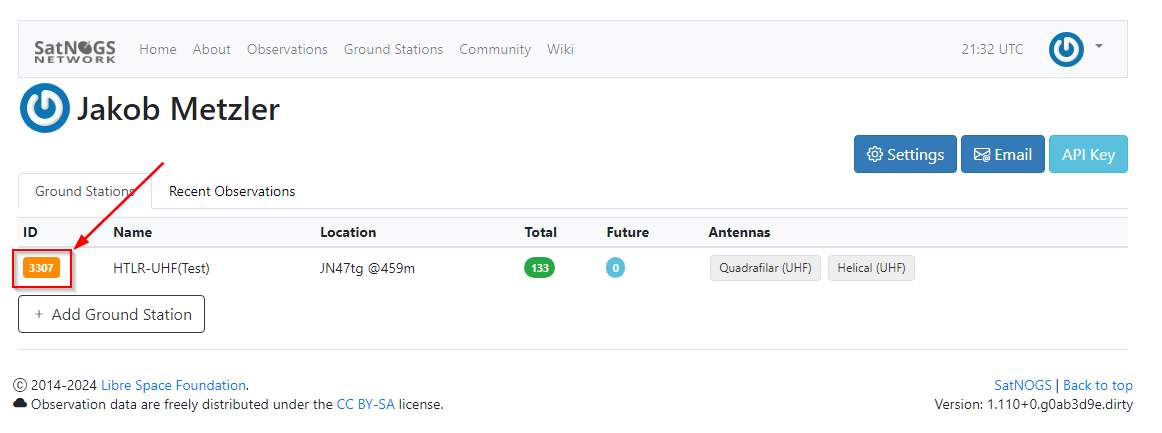
\includegraphics[width=.75\linewidth]{../ref/stationid.png}
	\caption{SatNOGS-Netzwerk Homepage: Station-ID ermitteln \cite{noauthor_satnogsdashboard_nodate}}
	\label{fig:stationid}
\end{figure}

\subsubsection{SATNOGS\textunderscore STATION\textunderscore LAT}
Dieser Parameter gibt den Breitengrad der Position der Empfangsstation an. Er wird für die Berechnungen der passierenden Satelliten und den dazugehörigen Elevation- und Azimutalwinkel verwendet.

\subsubsection{SATNOGS\textunderscore STATION\textunderscore LON}
Dieser Parameter gibt den Längengrad der Position der Empfangstation an. Er wird ebenfalls für die Berechnungen der passierenden Satelliten und den dazugehörigen Elevation- und Azimutalwinkel verwendet.

\section{Erweiterte Konfiguration} 
Wird im Hauptmenü der Reiter \glqq Advanced\grqq{} mit \glqq Enter\grqq{} ausgewählt, erscheint das folgende Fenster über welches erweiterte Einstellungen vorgenommen werden können. 

\begin{figure} [H]
	\centering
	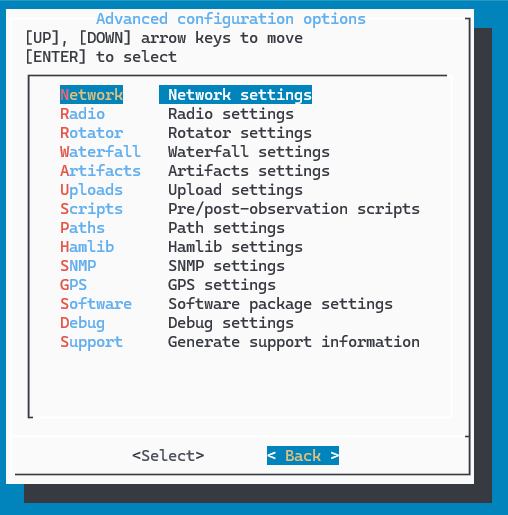
\includegraphics[width=.5\linewidth]{../ref/advanced_settings.png}
	\caption{SatNOGS Client: erweiterte Einstellungen}
	\label{fig:advanced_settings}
\end{figure}

Die wichtigsten Einstellungen, die hier vorgenommen werden können, sind das Definieren der Verstärkung des SDRs, das Einrichten einer Unterstützung für die Verwendung eines Rotors und das automatische Aktivieren von Bias-T während einer Observation.

\subsection{Verstärkung des SDRs einstellen}
Um die Verstärkung des SDRs einzustellen, müssen zuerst die möglichen Parameter ermittelt werden, was durch das Ausführen des Befehls \glqq rtl\textunderscore test\grqq{} in der SSH gemacht wird. 

\begin{figure} [H]
	\centering
	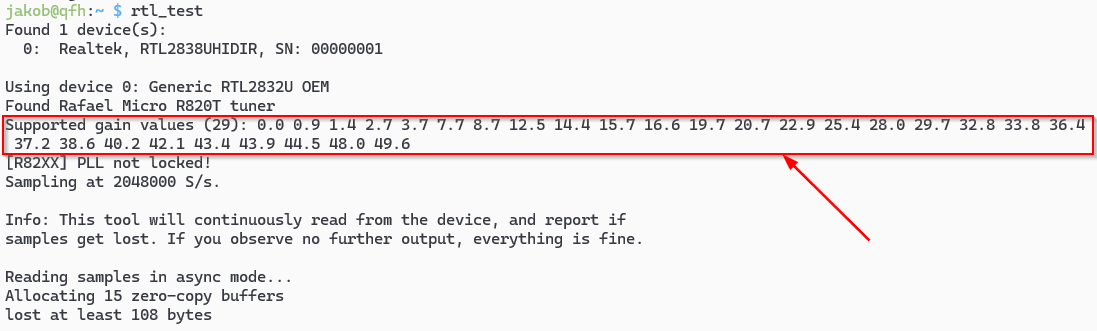
\includegraphics[width=\linewidth]{../ref/supportedgain.png}
	\caption{SatNOGS Client: unterstützte Gain Werte ermitteln}
	\label{fig:supportedgain}
\end{figure}

Wurde aus den ermittelten Gain Werten, wie in Abbildung \ref{fig:supportedgain} gezeigt, der gewünschte Wert der Verstärkung gewählt, so kann dieser in den erweiterten Einstellungen unter dem Reiter \glqq Radio\grqq{} mithilfe des Parameters \glqq SATNOGS\textunderscore RF\textunderscore GAIN\grqq{} eingestellt werden. 

\subsection{Rotor-Unterstützung implementieren}
Für die Implementierung einer Rotorsteuerung müssen in den erweiterten Einstellungen unter dem Reiter \glqq Rotator\grqq{} drei Parameter angepasst werden. 

Der erste Parameter \glqq{}SATNOGS\textunderscore ROT\textunderscore ENABLED\grqq{} aktiviert die Verwendung der konfigurierten Rotorsteuerung. 

Mithilfe des Parameters \glqq SATNOGS\textunderscore ROT\textunderscore MODEL\grqq{} wird das Model der Rotorsteuerung festgelegt. Im Fall der im Kapitel \ref{sec:gs232emulation} erläuterten GS232A/B Steuerung wird für den Parameter \glqq ROT\textunderscore MODEL\textunderscore GS232B\grqq{} verwendet \cite{noauthor_satnogsclient_nodate}. 

\glqq SATNOGS\textunderscore ROT\textunderscore BAUD\grqq{} legt die Baud-Rate der Kommunikation mit der Steuerung fest. Sie beträgt im Fall der im Kapitel \ref{sec:gs232emulation} erläuterten Steuerung 9600.

\subsection{Aktivieren von Bias-T}
Die Aktivierung von Bias-T ist abhängig vom verwendeten SDR. Sie wird nun nur für das RTL-SDR Blog v3 erläutert. Um die softwaremäßigen Voraussetzungen für die Verwendung von Bias-T am RTL-SDR Blog v3 zu erfüllen, müssen im ersten Schritt folgende Befehle in der SSH ausgeführt werden:
\newline 1. \glqq sudo apt install cmake\grqq{}
\newline 2. \glqq git clone https://github.com/rtlsdrblog/rtl\textunderscore biast\grqq{}
\newline 3. \glqq cd rtl\textunderscore biast\grqq{}
\newline 4. \glqq mkdir build\grqq{}
\newline 5. \glqq cd build\grqq{}
\newline 6. \glqq cmake ..\grqq{}
\newline 7. \glqq make\grqq{}

Diese Schritte ermöglichen die Kontrolle der Bias-T Funktion des RTL-SDR Blog v3 und müssen nur einmal durchgeführt werden. Bias-T kann nun über folgende Befehle manuell gesteuert werden:
\newline Einschalten: \glqq /rtl\textunderscore biast/build/src/rtl\textunderscore biast -b 1\grqq{}
\newline Ausschalten: \glqq /rtl\textunderscore biast/build/src/rtl\textunderscore biast -b 0\grqq{}

Diese Befehle können in den erweiterten Einstellungen unter dem Reiter Scripts als Pre- und Post-Observation Script festgelegt werden. Dazu wird der Einschalt- sowie Ausschalt-Befehl mit \glqq /home\grqq{} , aufgrund des Ursprungsverzeichnisses des SatNOGS Client, am Anfang erweitert. Somit wird Bias-T automatisch zum Startzeitpunkt einer Observation aktiviert und nach vollendeter Observation wieder deaktiviert. 